\documentclass[]{article}

\usepackage{xargs} 
\usepackage[colorinlistoftodos,prependcaption,textsize=tiny]{todonotes}
\newcommandx{\unsure}[2][1=]{\todo[linecolor=red,backgroundcolor=red!25,bordercolor=red,#1]{#2}}
\newcommandx{\change}[2][1=]{\todo[linecolor=blue,backgroundcolor=blue!25,bordercolor=blue,#1]{#2}}
\newcommandx{\info}[2][1=]{\todo[linecolor=OliveGreen,backgroundcolor=OliveGreen!25,bordercolor=OliveGreen,#1]{#2}}
\newcommandx{\improvement}[2][1=]{\todo[linecolor=purple,backgroundcolor=purple!25,bordercolor=purple,#1]{#2}}
\newcommandx{\thiswillnotshow}[2][1=]{\todo[disable,#1]{#2}}

\usepackage{enumitem}
\usepackage{multicol}

\usepackage{graphicx}
\usepackage{caption}
\usepackage{subcaption}

%opening
\title{}
\author{}

\begin{document}

\maketitle

\begin{abstract}

\end{abstract}

\section{Introduction}

\section{Related Work}

\section{Experiment Setup}

\todo{put a picture of the experiment setup here}

The multitouch user interface device used in this experiment is a 3M \todo{Exact model here} screen. 
This screen can track up to 20 simultaneous points, but reports only points, rather than shapes or areas of contact. \todo{pressure information? I think I had this in my initial drawing scripts}

Script read to each user to direct them to think aloud and use the user interface to direct the robots. 

While the user interacted with the touch screen, their touches and the positions of their hands were recorded by the computer connected to the screen and by the video cameras. 
One video camera was placed high, looking down at the screen, to track where the user's hand was on the screen. 
The other video camera was placed in front of the screen at a low angle, in order to observe whether the user's hands were touching the screen, or moving above it. 
In addition to touches and video, users were asked to think aloud about their actions.
This audio was recorded as well. 

The software used to record all of this information is ROS, the Robot Operating System \todo{cite}. 
ROS was developed as a message-passing framework for connecting modular programs on a robot \todo{explain better when not tired}. 
It may seem unusual to use a framework intended for operating robots as a recording program for collecting experiment data, but ROS provides a utility called rosbag that records some or all of the messages emitted by the robot's sensors in a ``bag'' file. 
In this case, the cameras, microphone, and UI application are the ``sensors'' for rosbag to record.
A ROS launch file starts multiple ROS nodes to record image data from the cameras, audio from the microphone, and touch events and screen updates from the UI.
ROS also provides tools for manipulating bag files, and playing them back. 
All of the data in the file is timestamped, so it plays back with the audio, video, and UI interactions all accurately synchronized. 
Because all of the data is treated as standard ROS message types, it is relatively easy to write custom processors for the recorded data.
For example, a node was written that accepts the replayed UI screen changes and touch events, and renders them as a stream of ROS image messages showing the contact points overlaid on the UI screen. 

\subsection{Experiment Conditions}

Users were given tasks in one of five conditions, varying by how many robots were in each condition. 
The conditions consisted of 1-2 robots, 10 robots, 100 robots, 1000 robots, or an unknown number of robots, represented by a cloud. 
For each condition, the user was requested to perform a sequence of tasks. 
The exact number of tasks varied between conditions due to some tasks not making sense with the number of robots involved. 

\begin{tabular}{l|l|l|l|l|l}
& 1 & 10 & 100 & 1000 & Unknown \\
Move to area A & x & x & x & x & x\\
Move to area A with a wall & x & x & x & x & x \\
Stop the robots & x & x & x & x & x\\
Divide around an obstacle & & x & x & x & x \\
Orange to B, red to A & x & x & x & x & x \\
Orange to A, red to B & x & x & x & x & x \\
Orange to A, red to B (mixed) & x & x & x & x & x \\
Divide group & x & x & x & x & x \\
Merge groups & & x & x & x & x \\
Form a line & & x & x & x & x \\
Form a square & & x & x & x & x \\
Move the crate to area A & x & x & x & x & x \\
Move the crate to area A (dispersed) & x & x & x & x & x\\
Mark defective robot & x & x & x & x & \\
Remove defective robot & x & x & x & x &  \\
Patrol the screen border & x & x & x & x & x \\
Patrol area A & x & x & x & x & x \\
Disperse over screen & x & x & x & x & x \\
\end{tabular}


The single robot case has 11 tasks:
\begin{enumerate}[noitemsep]
	\item Move to area A
	\item Move to area A with a wall in the way
	\item Stop the robot
	\item Orange robot to area A, red robot to area B
	\item Orange robot to area B, red robot to area A
	\item Divide group
	\item Move the crate to area A
	\item Mark defective robot \todo{check what people's interpretation of this is}
	\item Remove defective robot
	\item Patrol the screen border
	\item Patrol area A
\end{enumerate}

The 10, 100, and 1000 robot cases all have 18 tasks. The additional tasks are listed in bold:
\begin{enumerate}[noitemsep]
	\item Move to area A
	\item Move to area A with a wall in the way
	\item Stop the robots
	\item \textbf{Divide around an obstacle}
	\item Orange robots to area B, red robots to area A
	\item Orange robots to area A, red robots to area B
	\item \textbf{Orange robots to area A, red robots to area B (mixed color group)}
	\item Divide group
	\item \textbf{Merge groups}
	\item \textbf{Form a line}
	\item \textbf{Form a square}
	\item Move the crate to area A
	\item \textbf{Move the crate to area A (dispersed robots)}
	\item Mark defective robot \todo{check what people's interpretation of this is}
	\item Remove defective robot
	\item Patrol the screen border
	\item Patrol area A
\end{enumerate}

The additional tasks for the swarm robots are ones that don't make sense for individual robots, as a single robot cannot, for example, divide around an obstacle or form a square. The ``Merge groups" task was left out of the single robot case, because of the potential for confusion when referring to a ``group'' of one robot as a group. 

The unknown number of robots condition has 16 tasks. 
They are the same as the 10,100, and 1000 robot cases, but the ``Mark defective robot" and ``Remove defective robot" cases are omitted. 
Without UI elements that represent individual robots, the user cannot take any actions that refer to a specific robot. 


\section{Analysis}

User gestures were coded using a methodology adopted from the social sciences, Grounded Theory \todo{cite}.
Grounded Theory is an iterative process, where the data are first coded at a very fine-grained level, and then the resulting coded elements are compared to each other to try to determine their qualities, similarities, and differences. 
Codes can be consolidated or divided until repeated passes of coding and comparison no longer alter the emerging structure of the coding scheme. 
During each iteration of coding and comparison, the coder makes memos as well, describing the links they see between related coded elements and higher-level abstractions that relate the elements. 
These memos are eventually written up as the social scientific theory, which is believed to be grounded in the data because it arises from the coding process. 

We had NNN coders, and performed NNN \todo{I hope this is "2" at most} passes through the data.
After the first pass of coding, the coders met to compare memos and coding elements. During this meeting, we created a code book based on the codes that each coder developed \todo{This seems like kind of K-hacking}. All of the video was then recoded using the common codebook. 

[DATA INTENSIFIES]
 
Some people take the directions on the slides very literally. 
For example, users who had been solely using the touch interface read the slides that instructed "Tell the robots to form a line" to indicate that they should speak the words "Form a line", addressed to the robots.

People who didn't otherwise want voice commands would use them for the task of stopping the robots. 
Since this task assumes the robots are already moving towards a goal, attempts to interact with all of them while they are moving could be difficult. 

\subsection{Participant Demographics}

\section{Conclusions}

In future, it might be interesting to repeat this work with a condition that does not display the robots in the user interface at all. 
We expect that for conditions such as the ``move the crate'' tasks, the user would simply indicate the crate should move to area A, without concern for which robots perform the moving. 
However, such an interface would not afford indicating particular robots or groups, so tasks such as dividing the robots around an obstacle may become difficult to perform. 

\bibliography{../proposal/swarm.bib}
\bibliographystyle{apalike}

\section{Appendix of all Test Slides}
\begin{figure}
	\centering
	\begin{subfigure}{0.42\textwidth}
		\centering
		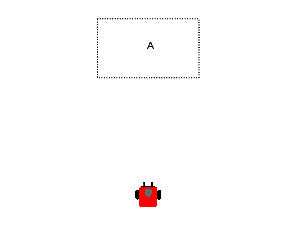
\includegraphics[width=\linewidth]{slide_images/Swarm_Robot_Control_-_Single_Robot_0003.png}
		\caption{Move to A}
		\label{fig:sub1}
	\end{subfigure}%
	\begin{subfigure}{0.42\textwidth}
		\centering
		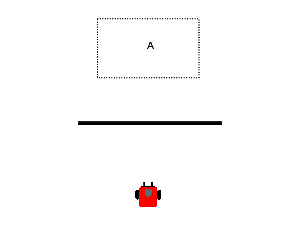
\includegraphics[width=\linewidth]{slide_images/Swarm_Robot_Control_-_Single_Robot_0005.png}
		\caption{Move to A with wall}
		\label{fig:sub2}
	\end{subfigure}
	\begin{subfigure}{0.42\textwidth}
		\centering
		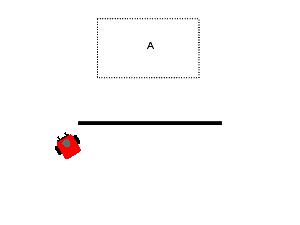
\includegraphics[width=\linewidth]{slide_images/Swarm_Robot_Control_-_Single_Robot_0007.png}
		\caption{Stop the robot}
		\label{fig:sub1}
	\end{subfigure}%
	\begin{subfigure}{0.42\textwidth}
		\centering
		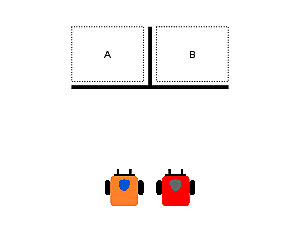
\includegraphics[width=\linewidth]{slide_images/Swarm_Robot_Control_-_Single_Robot_0009.png}
		\caption{Orange to B, Red to A}
		\label{fig:sub2}
	\end{subfigure}
	\begin{subfigure}{0.42\textwidth}
		\centering
		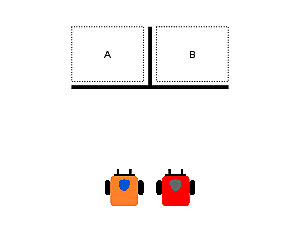
\includegraphics[width=\linewidth]{slide_images/Swarm_Robot_Control_-_Single_Robot_0011.png}
		\caption{Orange to A, Red to B}
		\label{fig:sub1}
	\end{subfigure}%
	\begin{subfigure}{0.42\textwidth}
		\centering
		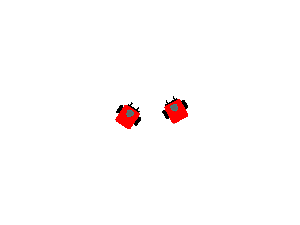
\includegraphics[width=\linewidth]{slide_images/Swarm_Robot_Control_-_Single_Robot_0013.png}
		\caption{Divide group}
		\label{fig:sub2}
	\end{subfigure}
	\begin{subfigure}{0.42\textwidth}
		\centering
		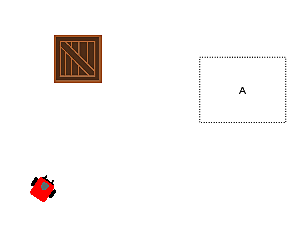
\includegraphics[width=\linewidth]{slide_images/Swarm_Robot_Control_-_Single_Robot_0015.png}
		\caption{Move the crate to A}
		\label{fig:sub1}
	\end{subfigure}%
	\begin{subfigure}{0.42\textwidth}
		\centering
		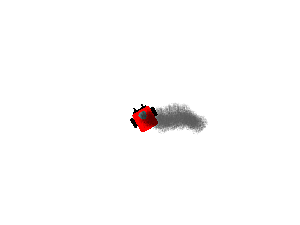
\includegraphics[width=\linewidth]{slide_images/Swarm_Robot_Control_-_Single_Robot_0017.png}
		\caption{Mark defective robot}
		\label{fig:sub2}
	\end{subfigure}
	\label{fig:single_robot_slides}
\end{figure}


\begin{figure}
	\ContinuedFloat
	\centering
	\begin{subfigure}{0.42\textwidth}
		\centering
		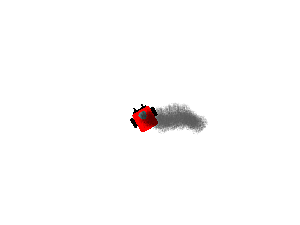
\includegraphics[width=\linewidth]{slide_images/Swarm_Robot_Control_-_Single_Robot_0019.png}
		\caption{Remove defective robot}
		\label{fig:sub1}
	\end{subfigure}%
	\begin{subfigure}{0.42\textwidth}
		\centering
		
\includegraphics[width=\linewidth]{slide_images/Swarm_Robot_Control_-_Single_Robot_0021.png}
		\caption{Patrol the screen border}
		\label{fig:sub2}
	\end{subfigure}
	\begin{subfigure}{0.42\textwidth}
		\centering
		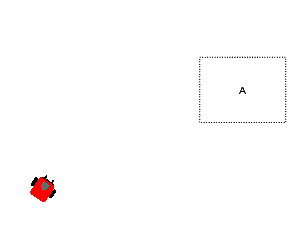
\includegraphics[width=\linewidth]{slide_images/Swarm_Robot_Control_-_Single_Robot_0023.png}
		\caption{Patrol area A}
		\label{fig:sub1}
	\end{subfigure}
	\label{fig:single_robot_slides_pt2}
\end{figure}


\begin{figure}
	\centering
	\begin{subfigure}{0.42\textwidth}
		\centering
		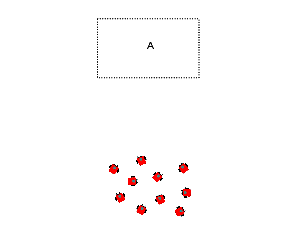
\includegraphics[width=\linewidth]{slide_images/Swarm_Robot_Control_-_10_Robot_0003.png}
		\caption{Move to A}
		\label{fig:sub1}
	\end{subfigure}%
	\begin{subfigure}{0.42\textwidth}
		\centering
		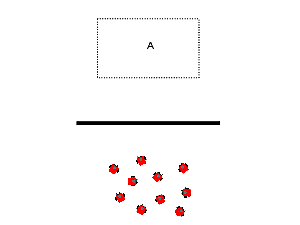
\includegraphics[width=\linewidth]{slide_images/Swarm_Robot_Control_-_10_Robot_0005.png}
		\caption{Move to A with wall}
		\label{fig:sub2}
	\end{subfigure}
	\begin{subfigure}{0.42\textwidth}
		\centering
		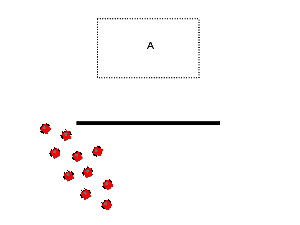
\includegraphics[width=\linewidth]{slide_images/Swarm_Robot_Control_-_10_Robot_0007.png}
		\caption{Stop the robots}
		\label{fig:sub1}
	\end{subfigure}%
	\begin{subfigure}{0.42\textwidth}
		\centering
		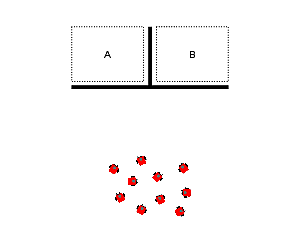
\includegraphics[width=\linewidth]{slide_images/Swarm_Robot_Control_-_10_Robot_0009.png}
		\caption{Divide around obstacle}
		\label{fig:sub2}
	\end{subfigure}
	\begin{subfigure}{0.42\textwidth}
		\centering
		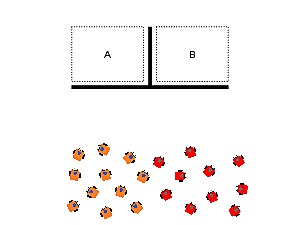
\includegraphics[width=\linewidth]{slide_images/Swarm_Robot_Control_-_10_Robot_0011.png}
		\caption{Orange to B, Red to A}
		\label{fig:sub1}
	\end{subfigure}%
	\begin{subfigure}{0.42\textwidth}
		\centering
		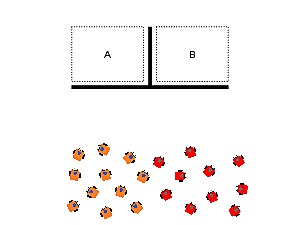
\includegraphics[width=\linewidth]{slide_images/Swarm_Robot_Control_-_10_Robot_0013.png}
		\caption{Orange to A, Red to B}
		\label{fig:sub2}
	\end{subfigure}
	\begin{subfigure}{0.42\textwidth}
		\centering
		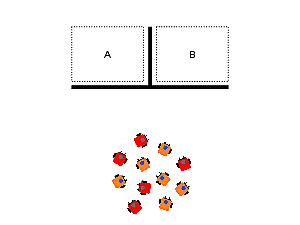
\includegraphics[width=\linewidth]{slide_images/Swarm_Robot_Control_-_10_Robot_0015.png}
		\caption{Orange to A, Red to B}
		\label{fig:sub1}
	\end{subfigure}%
	\begin{subfigure}{0.42\textwidth}
		\centering
		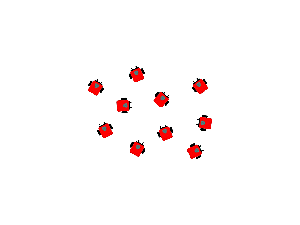
\includegraphics[width=\linewidth]{slide_images/Swarm_Robot_Control_-_10_Robot_0017.png}
		\caption{Divide group}
		\label{fig:sub2}
	\end{subfigure}
\end{figure}
	
	
\begin{figure}
	\ContinuedFloat
	\centering		
	\begin{subfigure}{0.42\textwidth}
		\centering
		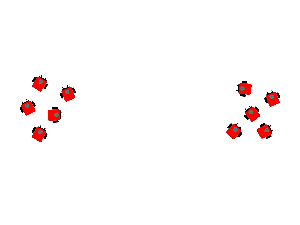
\includegraphics[width=\linewidth]{slide_images/Swarm_Robot_Control_-_10_Robot_0019.png}
		\caption{Combine groups}
		\label{fig:sub1}
	\end{subfigure}%
	\begin{subfigure}{0.42\textwidth}
		\centering
		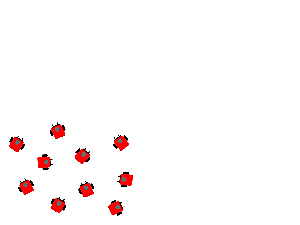
\includegraphics[width=\linewidth]{slide_images/Swarm_Robot_Control_-_10_Robot_0021.png}
		\caption{}
		\label{fig:sub2}
	\end{subfigure}
	\begin{subfigure}{0.42\textwidth}
		\centering
		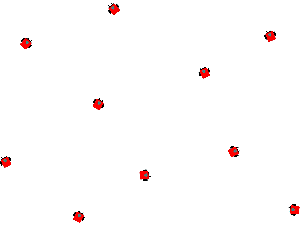
\includegraphics[width=\linewidth]{slide_images/Swarm_Robot_Control_-_10_Robot_0023.png}
		\caption{}
		\label{fig:sub1}
	\end{subfigure}%
	\begin{subfigure}{0.42\textwidth}
		\centering
		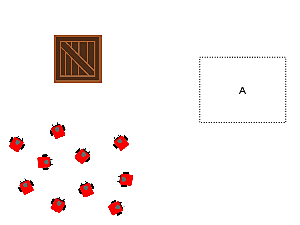
\includegraphics[width=\linewidth]{slide_images/Swarm_Robot_Control_-_10_Robot_0025.png}
		\caption{Orange to A, Red to B}
		\label{fig:sub1}
	\end{subfigure}
	\begin{subfigure}{0.42\textwidth}
		\centering
		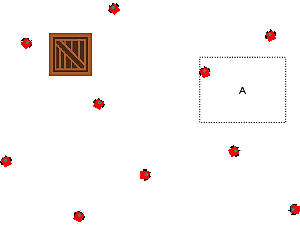
\includegraphics[width=\linewidth]{slide_images/Swarm_Robot_Control_-_10_Robot_0027.png}
		\caption{Divide group}
		\label{fig:sub2}
	\end{subfigure}%
	\begin{subfigure}{0.42\textwidth}
		\centering
		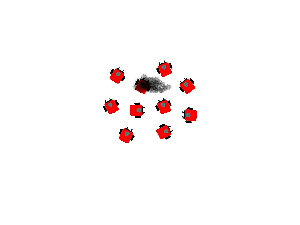
\includegraphics[width=\linewidth]{slide_images/Swarm_Robot_Control_-_10_Robot_0029.png}
		\caption{Combine groups}
		\label{fig:sub1}
	\end{subfigure}
	\begin{subfigure}{0.42\textwidth}
		\centering
		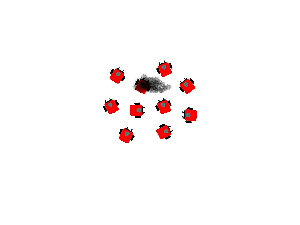
\includegraphics[width=\linewidth]{slide_images/Swarm_Robot_Control_-_10_Robot_0031.png}
		\caption{Form a line}
		\label{fig:sub2}
	\end{subfigure}%
	\begin{subfigure}{0.42\textwidth}
		\centering
		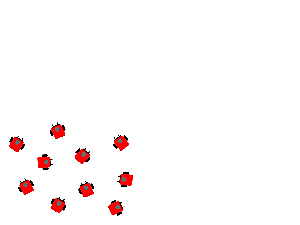
\includegraphics[width=\linewidth]{slide_images/Swarm_Robot_Control_-_10_Robot_0033.png}
		\caption{Form a square}
		\label{fig:sub1}
	\end{subfigure}
\end{figure}
	
	
\begin{figure}
	\ContinuedFloat
	\centering	
	\begin{subfigure}{0.42\textwidth}
		\centering
		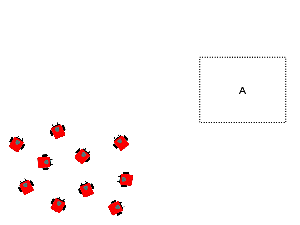
\includegraphics[width=\linewidth]{slide_images/Swarm_Robot_Control_-_10_Robot_0035.png}
		\caption{Move the crate to A}
		\label{fig:sub1}
	\end{subfigure}%
	\begin{subfigure}{0.42\textwidth}
		\centering
		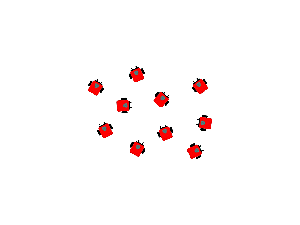
\includegraphics[width=\linewidth]{slide_images/Swarm_Robot_Control_-_10_Robot_0037.png}
		\caption{Move the crate to A}
		\label{fig:sub2}
	\end{subfigure}
	\label{fig:10_robot_slides}
\end{figure}

\begin{figure}
	\centering
	\begin{subfigure}{0.42\textwidth}
		\centering
		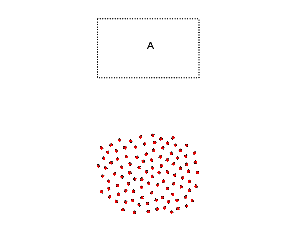
\includegraphics[width=\linewidth]{slide_images/Swarm_Robot_Control_-_100_Robot_0003.png}
		\caption{Move to A}
		\label{fig:sub1}
	\end{subfigure}%
	\begin{subfigure}{0.42\textwidth}
		\centering
		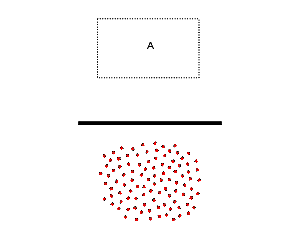
\includegraphics[width=\linewidth]{slide_images/Swarm_Robot_Control_-_100_Robot_0005.png}
		\caption{Move to A with wall}
		\label{fig:sub2}
	\end{subfigure}
	\begin{subfigure}{0.42\textwidth}
		\centering
		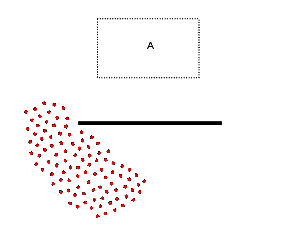
\includegraphics[width=\linewidth]{slide_images/Swarm_Robot_Control_-_100_Robot_0007.png}
		\caption{Stop the robots}
		\label{fig:sub1}
	\end{subfigure}%
	\begin{subfigure}{0.42\textwidth}
		\centering
		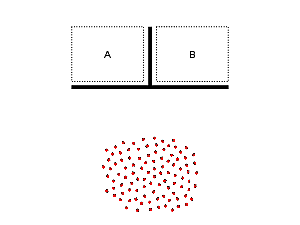
\includegraphics[width=\linewidth]{slide_images/Swarm_Robot_Control_-_100_Robot_0009.png}
		\caption{Divide around obstacle}
		\label{fig:sub2}
	\end{subfigure}
	\begin{subfigure}{0.42\textwidth}
		\centering
		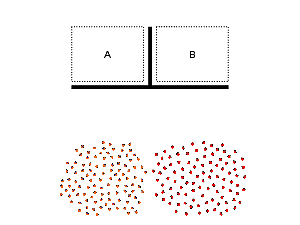
\includegraphics[width=\linewidth]{slide_images/Swarm_Robot_Control_-_100_Robot_0011.png}
		\caption{Orange to B, Red to A}
		\label{fig:sub1}
	\end{subfigure}%
	\begin{subfigure}{0.42\textwidth}
		\centering
		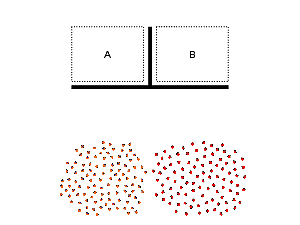
\includegraphics[width=\linewidth]{slide_images/Swarm_Robot_Control_-_100_Robot_0013.png}
		\caption{Orange to A, Red to B}
		\label{fig:sub2}
	\end{subfigure}
	\begin{subfigure}{0.42\textwidth}
		\centering
		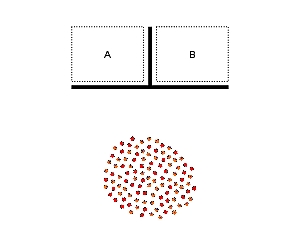
\includegraphics[width=\linewidth]{slide_images/Swarm_Robot_Control_-_100_Robot_0015.png}
		\caption{Orange to A, Red to B}
		\label{fig:sub1}
	\end{subfigure}%
	\begin{subfigure}{0.42\textwidth}
		\centering
		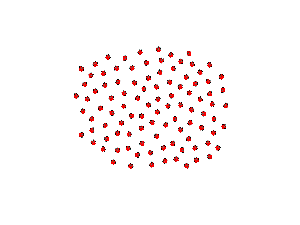
\includegraphics[width=\linewidth]{slide_images/Swarm_Robot_Control_-_100_Robot_0017.png}
		\caption{Divide group}
		\label{fig:sub2}
	\end{subfigure}
\end{figure}
\begin{figure}
	\ContinuedFloat
	\centering
	\begin{subfigure}{0.42\textwidth}
		\centering
		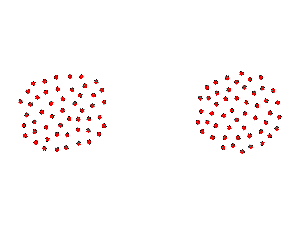
\includegraphics[width=\linewidth]{slide_images/Swarm_Robot_Control_-_100_Robot_0019.png}
		\caption{Combine groups}
		\label{fig:sub1}
	\end{subfigure}%
	\begin{subfigure}{0.42\textwidth}
		\centering
		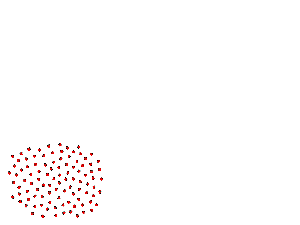
\includegraphics[width=\linewidth]{slide_images/Swarm_Robot_Control_-_100_Robot_0021.png}
		\caption{Form a line}
		\label{fig:sub2}
	\end{subfigure}
	\begin{subfigure}{0.42\textwidth}
		\centering
		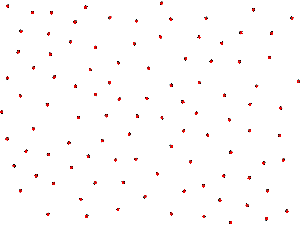
\includegraphics[width=\linewidth]{slide_images/Swarm_Robot_Control_-_100_Robot_0023.png}
		\caption{Form a square}
		\label{fig:sub1}
	\end{subfigure}%
	\begin{subfigure}{0.42\textwidth}
		\centering
		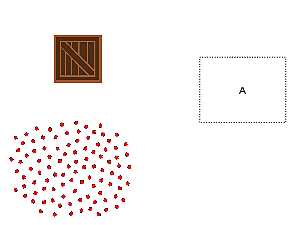
\includegraphics[width=\linewidth]{slide_images/Swarm_Robot_Control_-_100_Robot_0025.png}
		\caption{Move the crate to area A}
		\label{fig:sub1}
	\end{subfigure}
	\begin{subfigure}{0.42\textwidth}
		\centering
		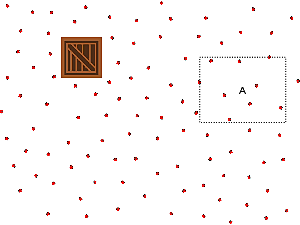
\includegraphics[width=\linewidth]{slide_images/Swarm_Robot_Control_-_100_Robot_0027.png}
		\caption{Move the crate to area A}
		\label{fig:sub2}
	\end{subfigure}%
	\begin{subfigure}{0.42\textwidth}
		\centering
		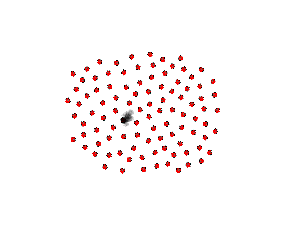
\includegraphics[width=\linewidth]{slide_images/Swarm_Robot_Control_-_100_Robot_0029.png}
		\caption{Mark defective robot}
		\label{fig:sub1}
	\end{subfigure}
	\begin{subfigure}{0.42\textwidth}
		\centering
		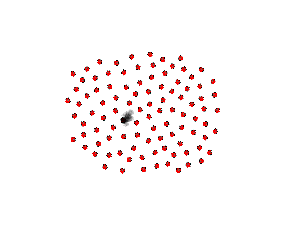
\includegraphics[width=\linewidth]{slide_images/Swarm_Robot_Control_-_100_Robot_0031.png}
		\caption{Remove defective robot}
		\label{fig:sub2}
	\end{subfigure}%
	\begin{subfigure}{0.42\textwidth}
		\centering
		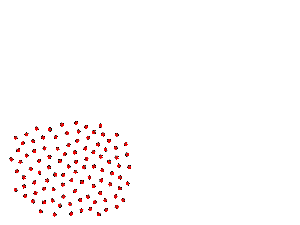
\includegraphics[width=\linewidth]{slide_images/Swarm_Robot_Control_-_100_Robot_0033.png}
		\caption{Patrol the screen border}
		\label{fig:sub1}
	\end{subfigure}
\end{figure}
\begin{figure}
	\ContinuedFloat
	\centering	
		\begin{subfigure}{0.42\textwidth}
		\centering
		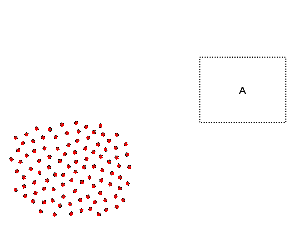
\includegraphics[width=\linewidth]{slide_images/Swarm_Robot_Control_-_100_Robot_0035.png}
		\caption{Patrol area A}
		\label{fig:sub1}
	\end{subfigure}%
	\begin{subfigure}{0.42\textwidth}
		\centering
		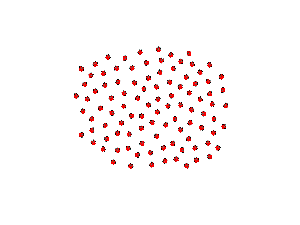
\includegraphics[width=\linewidth]{slide_images/Swarm_Robot_Control_-_100_Robot_0037.png}
		\caption{Disperse over screen}
		\label{fig:sub2}
	\end{subfigure}
	\label{fig:100_robot_slides}
\end{figure}


\begin{figure}
	\centering
	\begin{subfigure}{0.42\textwidth}
		\centering
		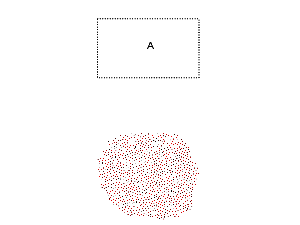
\includegraphics[width=\linewidth]{slide_images/Swarm_Robot_Control_-_1000_Robot_0003.png}
		\caption{Move to A}
		\label{fig:sub1}
	\end{subfigure}%
	\begin{subfigure}{0.42\textwidth}
		\centering
		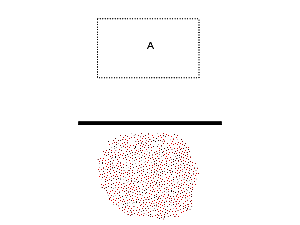
\includegraphics[width=\linewidth]{slide_images/Swarm_Robot_Control_-_1000_Robot_0005.png}
		\caption{Move to A with wall}
		\label{fig:sub2}
	\end{subfigure}
	\begin{subfigure}{0.42\textwidth}
		\centering
		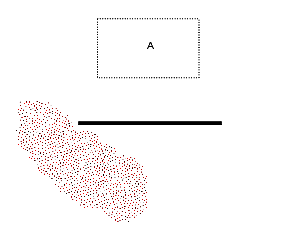
\includegraphics[width=\linewidth]{slide_images/Swarm_Robot_Control_-_1000_Robot_0007.png}
		\caption{Stop the robots}
		\label{fig:sub1}
	\end{subfigure}%
	\begin{subfigure}{0.42\textwidth}
		\centering
		\includegraphics[width=\linewidth]{slide_images/Swarm_Robot_Control_-_1000_Robot_0009.png}
		\caption{Divide around obstacle}
		\label{fig:sub2}
	\end{subfigure}
	\begin{subfigure}{0.42\textwidth}
		\centering
		\includegraphics[width=\linewidth]{slide_images/Swarm_Robot_Control_-_1000_Robot_0011.png}
		\caption{Orange to B, Red to A}
		\label{fig:sub1}
	\end{subfigure}%
	\begin{subfigure}{0.42\textwidth}
		\centering
		\includegraphics[width=\linewidth]{slide_images/Swarm_Robot_Control_-_1000_Robot_0013.png}
		\caption{Orange to A, Red to B}
		\label{fig:sub2}
	\end{subfigure}
	\begin{subfigure}{0.42\textwidth}
		\centering
		\includegraphics[width=\linewidth]{slide_images/Swarm_Robot_Control_-_1000_Robot_0015.png}
		\caption{Orange to A, Red to B}
		\label{fig:sub1}
	\end{subfigure}%
	\begin{subfigure}{0.42\textwidth}
		\centering
		\includegraphics[width=\linewidth]{slide_images/Swarm_Robot_Control_-_1000_Robot_0017.png}
		\caption{Divide group}
		\label{fig:sub2}
	\end{subfigure}
\end{figure}
\begin{figure}
	\ContinuedFloat
	\centering
	\begin{subfigure}{0.42\textwidth}
		\centering
		\includegraphics[width=\linewidth]{slide_images/Swarm_Robot_Control_-_1000_Robot_0019.png}
		\caption{Combine groups}
		\label{fig:sub1}
	\end{subfigure}%
	\begin{subfigure}{0.42\textwidth}
		\centering
		\includegraphics[width=\linewidth]{slide_images/Swarm_Robot_Control_-_1000_Robot_0021.png}
		\caption{Form a line}
		\label{fig:sub2}
	\end{subfigure}
	\begin{subfigure}{0.42\textwidth}
		\centering
		\includegraphics[width=\linewidth]{slide_images/Swarm_Robot_Control_-_1000_Robot_0023.png}
		\caption{Form a square}
		\label{fig:sub1}
	\end{subfigure}%
	\begin{subfigure}{0.42\textwidth}
		\centering
		\includegraphics[width=\linewidth]{slide_images/Swarm_Robot_Control_-_1000_Robot_0025.png}
		\caption{Move the crate to area A}
		\label{fig:sub1}
	\end{subfigure}
	\begin{subfigure}{0.42\textwidth}
		\centering
		\includegraphics[width=\linewidth]{slide_images/Swarm_Robot_Control_-_1000_Robot_0027.png}
		\caption{Move the crate to area A}
		\label{fig:sub2}
	\end{subfigure}%
	\begin{subfigure}{0.42\textwidth}
		\centering
		\includegraphics[width=\linewidth]{slide_images/Swarm_Robot_Control_-_1000_Robot_0029.png}
		\caption{Mark defective robot}
		\label{fig:sub1}
	\end{subfigure}
	\begin{subfigure}{0.42\textwidth}
		\centering
		\includegraphics[width=\linewidth]{slide_images/Swarm_Robot_Control_-_1000_Robot_0031.png}
		\caption{Remove defective robot}
		\label{fig:sub2}
	\end{subfigure}%
	\begin{subfigure}{0.42\textwidth}
		\centering
		\includegraphics[width=\linewidth]{slide_images/Swarm_Robot_Control_-_1000_Robot_0033.png}
		\caption{Patrol the screen border}
		\label{fig:sub1}
	\end{subfigure}
\end{figure}
\begin{figure}
	\ContinuedFloat
	\centering	
		\begin{subfigure}{0.42\textwidth}
		\centering
		\includegraphics[width=\linewidth]{slide_images/Swarm_Robot_Control_-_1000_Robot_0035.png}
		\caption{Patrol area A}
		\label{fig:sub1}
	\end{subfigure}%
	\begin{subfigure}{0.42\textwidth}
		\centering
		\includegraphics[width=\linewidth]{slide_images/Swarm_Robot_Control_-_1000_Robot_0037.png}
		\caption{Disperse over screen}
		\label{fig:sub2}
	\end{subfigure}
	\label{fig:1000_robot_slides}
\end{figure}



\begin{figure}
	\centering
	\begin{subfigure}{0.42\textwidth}
		\centering
		\includegraphics[width=\linewidth]{slide_images/Swarm_Robot_Control_-_Unknown_Number_of_Robots_0005.png}
		\caption{Move to A}
		\label{fig:sub1}
	\end{subfigure}%
	\begin{subfigure}{0.42\textwidth}
		\centering
		\includegraphics[width=\linewidth]{slide_images/Swarm_Robot_Control_-_Unknown_Number_of_Robots_0007.png}
		\caption{Move to A with wall}
		\label{fig:sub2}
	\end{subfigure}
	\begin{subfigure}{0.42\textwidth}
		\centering
		\includegraphics[width=\linewidth]{slide_images/Swarm_Robot_Control_-_Unknown_Number_of_Robots_0009.png}
		\caption{Stop the robots}
		\label{fig:sub1}
	\end{subfigure}%
	\begin{subfigure}{0.42\textwidth}
		\centering
		\includegraphics[width=\linewidth]{slide_images/Swarm_Robot_Control_-_Unknown_Number_of_Robots_0011.png}
		\caption{Divide around obstacle}
		\label{fig:sub2}
	\end{subfigure}
	\begin{subfigure}{0.42\textwidth}
		\centering
		\includegraphics[width=\linewidth]{slide_images/Swarm_Robot_Control_-_Unknown_Number_of_Robots_0013.png}
		\caption{Orange to B, Red to A}
		\label{fig:sub1}
	\end{subfigure}%
	\begin{subfigure}{0.42\textwidth}
		\centering
		\includegraphics[width=\linewidth]{slide_images/Swarm_Robot_Control_-_Unknown_Number_of_Robots_0015.png}
		\caption{Orange to A, Red to B}
		\label{fig:sub2}
	\end{subfigure}
	\begin{subfigure}{0.42\textwidth}
		\centering
		\includegraphics[width=\linewidth]{slide_images/Swarm_Robot_Control_-_Unknown_Number_of_Robots_0017.png}
		\caption{Orange to A, Red to B}
		\label{fig:sub1}
	\end{subfigure}%
	\begin{subfigure}{0.42\textwidth}
		\centering
		\includegraphics[width=\linewidth]{slide_images/Swarm_Robot_Control_-_Unknown_Number_of_Robots_0019.png}
		\caption{Divide group}
		\label{fig:sub2}
	\end{subfigure}
\end{figure}
\begin{figure}
	\ContinuedFloat
	\centering
	\begin{subfigure}{0.42\textwidth}
		\centering
		\includegraphics[width=\linewidth]{slide_images/Swarm_Robot_Control_-_Unknown_Number_of_Robots_0021.png}
		\caption{Combine groups}
		\label{fig:sub1}
	\end{subfigure}%
	\begin{subfigure}{0.42\textwidth}
		\centering
		\includegraphics[width=\linewidth]{slide_images/Swarm_Robot_Control_-_Unknown_Number_of_Robots_0023.png}
		\caption{Form a line}
		\label{fig:sub2}
	\end{subfigure}
	\begin{subfigure}{0.42\textwidth}
		\centering
		\includegraphics[width=\linewidth]{slide_images/Swarm_Robot_Control_-_Unknown_Number_of_Robots_0025.png}
		\caption{Form a square}
		\label{fig:sub1}
	\end{subfigure}%
	\begin{subfigure}{0.42\textwidth}
		\centering
		\includegraphics[width=\linewidth]{slide_images/Swarm_Robot_Control_-_Unknown_Number_of_Robots_0027.png}
		\caption{Move the crate to area A}
		\label{fig:sub1}
	\end{subfigure}
	\begin{subfigure}{0.42\textwidth}
		\centering
		\includegraphics[width=\linewidth]{slide_images/Swarm_Robot_Control_-_Unknown_Number_of_Robots_0029.png}
		\caption{Move the crate to area A}
		\label{fig:sub2}
	\end{subfigure}%
	\begin{subfigure}{0.42\textwidth}
		\centering
		\includegraphics[width=\linewidth]{slide_images/Swarm_Robot_Control_-_Unknown_Number_of_Robots_0031.png}
		\caption{Patrol the screen border}
		\label{fig:sub1}
	\end{subfigure}
	\begin{subfigure}{0.42\textwidth}
		\centering
		\includegraphics[width=\linewidth]{slide_images/Swarm_Robot_Control_-_Unknown_Number_of_Robots_0033.png}
		\caption{Patrol area A}
		\label{fig:sub2}
	\end{subfigure}%
	\begin{subfigure}{0.42\textwidth}
		\centering
		\includegraphics[width=\linewidth]{slide_images/Swarm_Robot_Control_-_Unknown_Number_of_Robots_0035.png}
		\caption{Disperse over the screen area}
		\label{fig:sub1}
	\end{subfigure}
\end{figure}

\end{document}
